\begin{frame}
    \frametitle{Viagem no tempo}

    \alert{\Large É possível viajar no tempo?}

    \uncover<2->{Resposta curta: {\bfseries sim!}}
    \begin{itemize}
        \item<3-> Para o futuro: \uncover<4->{\em viver}
        \item<3-> Para o passado: \uncover<5->{\em lembrar}
    \end{itemize}
\end{frame}

\begin{frame}
    \frametitle{Viagem no tempo}

    {\Large É possível viajar no tempo \alert{fora do trivial}?}

    \uncover<2->{Resposta curta: {\bfseries talvez...}}
\end{frame}

\subsection{Viagem ao futuro}

\begin{frame}
    \frametitle{Segundo a Física Clássica}

    \begin{block}{Física Newtoniana}
        \begin{itemize}
            \item Tempo é absoluto
            \begin{itemize}
                \item Noção de ``relógio global''.
                \item Passagem do tempo acontece na mesma proporção para todos os lugares do universo.
            \end{itemize}
            \item Tempo é irrefreável
            \begin{itemize}
                \item ``O espaço'' acontece várias e várias vezes, e o que usamos para rotular as ocorrências é ``o tempo''.
                \note[item]{Espaço-tempo como um filme de projetor.}
            \end{itemize}
        \end{itemize}
    \end{block}
    \only<2->{De uma certa forma, a viagem no tempo não se sustenta no mundo Newtoniano.}
\end{frame}

\begin{frame}
    \frametitle{Segundo a Física Moderna}
    
    \begin{block}{Relatividade Restrita}
        \begin{itemize}
            \item Tempo é relativo
            \item Tempo é influenciado pela velocidade
        \end{itemize}
    \end{block}
\end{frame}

\begin{frame}
    \frametitle{Segundo a Física Moderna}
    
    \begin{block}{Relatividade Geral}
        \begin{itemize}
            \item Tempo é relativo
            \item Tempo é influenciado pela velocidade
            \item Tempo é influenciado pela gravidade
        \end{itemize}
    \end{block}
\end{frame}

\begin{frame}
    \frametitle{Segundo a Física Moderna -- Relatividade Geral}
    
    \begin{block}{Viagem ao futuro é possível}
        \begin{itemize}
            \item Experimentar um campo gravitacional menor.
            \item Experimentar velocidades extremas.
        \end{itemize}
    \end{block}

    \uncover<2->{
        \begin{block}{Paradoxo do Gêmeo}
            \centering
            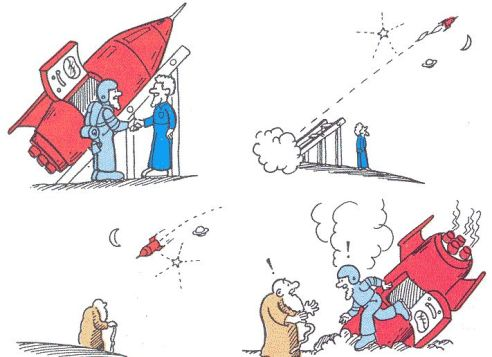
\includegraphics[width=0.65\textwidth]{img/twin_paradox.jpg}
        \end{block}
    }
\end{frame}

\begin{frame}
    \frametitle{Segundo a Física Moderna -- Relatividade Geral}
    
    \centering
    \transparent{0}\includegraphics[width=0.5\textwidth]{example-image}

    \note[item]{Do ponto de vista de um observador na origem, o deslocamento no eixo y ficou mais lento.}
    \note[item]{Do ponto de vista de um observador na origem, o tempo para o viagente passou mais lentamente.}
    \note[item]{Do ponto de vista do viajante, nada mudou.}
\end{frame}

\begin{frame}
    \frametitle{Segundo a Física Moderna -- Relatividade Geral}
    
    A gravidade é capaz de distorcer o {\em continuum} espaço-tempo.~\cite{visual-gravidade}
    
    \centering
    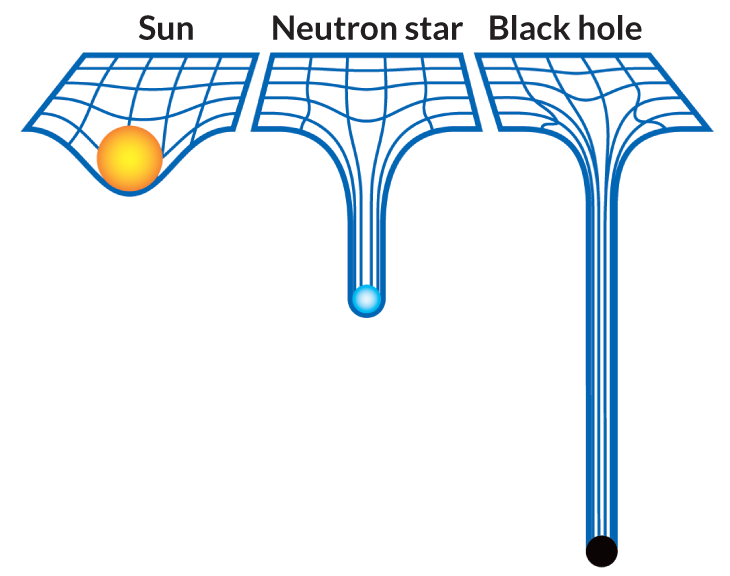
\includegraphics[width=0.6\textwidth]{img/continuum_distortion.png}

    \note[item]{O espaço-tempo foi menos esticado pelo campo gravitacional do objeto mais leve e mais pelo mais pesado.}
    \note[item]{Como se, do ponto de vista de quem ficou, quem foi fez o percurso em menos tempo.}
    \note[item]{Observável nos satélites que orbitam a terra. Necessária correção para funcionamento do GPS, por exemplo.}
\end{frame}

\begin{frame}
    \frametitle{Segundo a Física Moderna -- Relatividade Geral}
    
    \begin{block}{Viagem ao futuro é possível}
        \begin{itemize}
            \item Ponte de Einstein-Rosen. (buraco de minhoca)
        \end{itemize}
    \end{block}

    \centering
    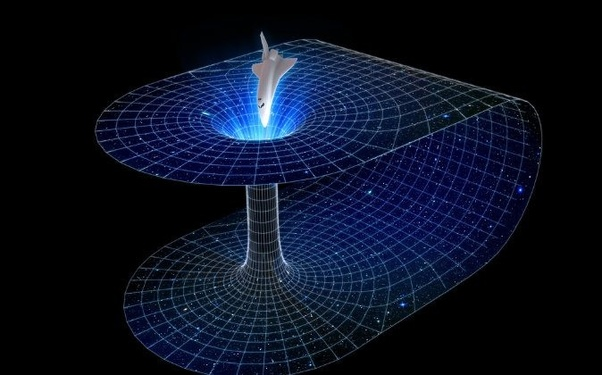
\includegraphics[height=0.6\textwidth]{img/wormhole.jpg}
    
\end{frame}

\begin{frame}
    \frametitle{Segundo a Física Moderna -- Relatividade Geral}
    
    \centering
    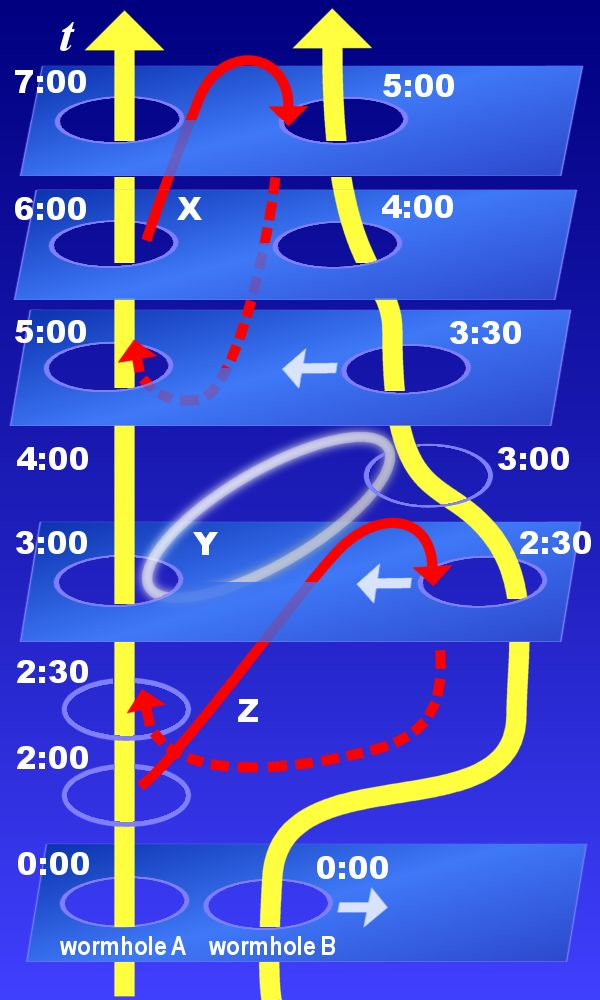
\includegraphics[height=0.75\textwidth]{img/wormhole_timetravel.jpg}
    
\end{frame}

\begin{frame}
    \frametitle{Então...}

    \alert{Dá pra viajar no tempo!} \uncover<2->{Mas dá mesmo...?}

    \begin{itemize}[<3->]
        \item Todas as soluções parecem requerer:
        \begin{itemize}
            \item Energia infinita
            \item Espaço infinito
            \item Massa negativa
        \end{itemize}
        \item<4-> E quase sempre o resultado disso termina na criação de um buraco-negro...
    \end{itemize}
\end{frame}

\subsection{Viagem ao passado}

\begin{frame}
    \frametitle{Então...}

    O problema mesmo é \alert{viajar para o passado...}
\end{frame}

\begin{frame}
    \frametitle{Paradoxos}
    
    \begin{block}{Paradoxo do Avô}
        \centering
        \transparent{0}\includegraphics[width=0.5\textwidth]{example-image}
    \end{block}

    \begin{itemize}
        \item<2-> Se eu puder voltar ao passado, para antes dos meus avós se conhecerem,
        \item<3-> encontrar e matar meu avô,
        \item<4-> eu não poderia existir.
        \item<5-> {\bfseries Mas como eu poderia ter voltado para impedi-los de se conhecer?} 
    \end{itemize}
    
    \note[item]{Contado em algumas versões, incluindo pai ou impedir sua própria viagem.}
    
\end{frame}

\begin{frame}
    \frametitle{Paradoxos}
    
    \begin{block}{Paradoxo da Predestinação}
        \centering
        \transparent{0}\includegraphics[width=0.5\textwidth]{example-image}
    \end{block}

    \begin{itemize}
        \item {\bfseries Ou será que os acontecimentos estão predestinados?}
    \end{itemize}
    
\end{frame}

\begin{frame}
    \frametitle{Paradoxos}
    
    \begin{block}{Paradoxo da Informação sem Fonte}
        \centering
        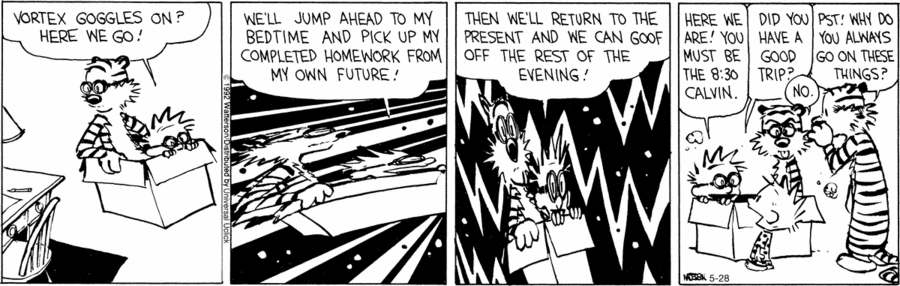
\includegraphics[width=\textwidth]{img/calvin_hobbes.png}
    \end{block}

    \begin{itemize}
        \item<2-> Se o Calvin das 8h30 possui o dever de casa feito,
        \item<3-> e o do passado puder pegar e voltar para curtir a tarde,
        \item<4-> para às 8h30 entregar o dever ao que veio do passado,
        \item<5-> {\bfseries quem fez o dever?}
    \end{itemize}
    \note[item]{Contado em algumas versões, incluindo Leonardo Da Vinci e a Mona Lisa.}
    
\end{frame}

\begin{frame}
    \frametitle{E agora?}
    
    \begin{itemize}
        \item Ao menos três teorias são possíveis:
        \begin{itemize}[<+->]
            \item Princípio da Autoconsistência de Novikov
            \item Predestinação
            \item Multiverso
        \end{itemize}
        \item<+-> Mesmo assim, ainda não se imagina como voltar para antes do momento da criação da máquina a ser usada.
        \note[item]{Frase de Stephen King: ``A viagem sendo possível, onde estão os viajantes?''}
    \end{itemize}
\end{frame}